\documentclass[aspectratio=169]{beamer}

\usetheme{upc}

\usepackage{etex}
\usepackage{pgf,pgfopts,pgfplots}
\usepackage{mathrsfs}
\usepackage{tikz-uml}

\pgfplotsset{compat=1.10}

\title{Algoritmos y Estructuras de Datos}
\subtitle{Introducción a las Estructuras de Datos y Algoritmos}
\date{2015}
\institute{\href{http://www.upc.edu.pe}{Universidad Peruana de Ciencias Aplicadas}}

\begin{document}

\maketitle

\begin{frame}{Outline}
  \tableofcontents
\end{frame}

%%%%%%%%%%%%%%%%%%%% Primera sección %%%%%%%%%%%%%%%%%%%%%%%%%%%%%%
\section{Tipos de datos abstractos}

\begin{frame}{Computerphile}

\begin{block}{Dr. James Clewett}
\href{https://www.youtube.com/watch?v=p7nGcY73epw}{The Art of Abstraction}

https://www.youtube.com/watch?v=p7nGcY73epw
\end{block}

\end{frame}

\begin{frame}{Definición}

\begin{block}{Abstracción}
Es el proceso de quitar características de algo para reducir su complejidad.
\end{block}

\begin{block}{Tipo de dato}
Un tipo particular de ítem, definido por los valores que éste puede tomar, el lenguaje de programación usado o las operaciones que se realizan sobre éste.
\end{block}

\end{frame}

\begin{frame}{Tipos de abstracción}

\begin{block}{Lenguajes de programación}
Assembler, Lenguajes orientados a objetos, lenguajes lógicos, funcionales (lambdas y funciones de primera clase, por ejemplo, se tratarán posteriormente en el curso), etc.
\end{block}

\begin{block}{Control de flujo}
Programación estructurada, estructuras de control, etc.
\end{block}

\begin{block}{De datos}
Tipos de datos y tipos de datos abstractos como Registros, Clases, Interfaces, etc.
\end{block}

\end{frame}

\begin{frame}{Programación orientada a objetos}
  \begin{enumerate}
    \item ¿Qué es un objeto?
    \item ¿Qué es una clase?
    \item ¿Qué es encapsulamiento?
    \item ¿Qué es herencia?
    \item ¿Qué es polimorfismo?
    \item ¿Cuales son los tipos de relaciones entre clases más importantes?
  \end{enumerate}
\end{frame}

\begin{frame}{Diagramas de clases}
  \begin{itemize}
    \item modificadorAcceso nombreAtributo: tipoDato
    \item modificadorAcceso nombreMetodo(atributos): tipoDato
  \end{itemize}
  \begin{center}
    
\begin{tikzpicture}
      \umlclass{SomeClass}{
        -- privateStuff : string \\
        \# protectedStuff : char \\
        $\sim$ packageAccess : int \\
        \umlstatic{-- staticStuff: long}
      }{
        + publicMethod() : bool \\
        \umlvirt{+ virtualMethod() : void}
      }
    \end{tikzpicture}
  \end{center}
\end{frame}

\begin{frame}{Diagramas de clases}
  \begin{center}
    \begin{tikzpicture}
      \umlemptyclass{A}
      \umlemptyclass[x=4]{B}
      \umluniassoc[arg2=rol,mult1=1,mult2=1..*]{A}{B}
    \end{tikzpicture}
    \begin{tabu}{|l|l|}
      \hline
      \rowfont[c]{\bfseries} Multiplicidad & Nomenclatura \\ \hline
      Sólo 1 & 1 \\ \hline
      Cero o uno & 0..1 \\ \hline
      Cero o más & 0..* \\ \hline
      Uno o más & 1..* \\ \hline
    \end{tabu}
  \end{center}
\end{frame}

\begin{frame}{Diagramas de clases}
  \begin{center}
    \begin{tikzpicture}
      \umlemptyclass{A}
      \umlemptyclass[x=4]{B}
      \umlcompo[]{A}{B}
    \end{tikzpicture}
    \begin{tikzpicture}
      \umlemptyclass{A}
      \umlemptyclass[x=4]{B}
      \umlunicompo[]{A}{B}
    \end{tikzpicture}
  \end{center}
  \begin{center}
    Composición
  \end{center}
  \begin{center}
    \begin{tikzpicture}
      \umlemptyclass{A}
      \umlemptyclass[x=4]{B}
      \umlaggreg[]{A}{B}
    \end{tikzpicture}
    \begin{tikzpicture}
      \umlemptyclass{A}
      \umlemptyclass[x=4]{B}
      \umluniaggreg[]{A}{B}
    \end{tikzpicture}
  \end{center}
  \begin{center}
    Agregación
  \end{center}
\end{frame}

\begin{frame}{Diagramas de clases}
  \begin{center}
    \begin{tikzpicture}
      \umlemptyclass{A}
      \umlemptyclass[x=4]{B}
      \umlassoc[]{A}{B}
    \end{tikzpicture}
    \begin{tikzpicture}
      \umlemptyclass{A}
      \umlemptyclass[x=4]{B}
      \umluniassoc[]{A}{B}
    \end{tikzpicture}
  \end{center}
  \begin{center}
    Asociación
  \end{center}
  \begin{center}
    \begin{tikzpicture}
      \umlemptyclass{A}
      \umlemptyclass[x=4]{B}
      \umldep[]{A}{B}
    \end{tikzpicture}
  \end{center}
  \begin{center}
    Dependencia
  \end{center}
\end{frame}

\begin{frame}{Diagramas de clases}
\begin{columns}
  \column{.5\textwidth}
  \begin{center}
    \begin{tikzpicture}
      \umlemptyclass{A}
      \umlemptyclass[x=4]{B}
      \umlinherit[]{A}{B}
    \end{tikzpicture}
  \end{center}
  \begin{center}
    Herencia
  \end{center}
  \column{.5\textwidth}
  \begin{center}
    \begin{tikzpicture}
      \umlemptyclass[x=-4]{A}
      \umlemptyclass[type=interface]{B}
      \umlreal[]{A}{B}
    \end{tikzpicture}
  \end{center}
  \begin{center}
    Realización
  \end{center}
\end{columns}
\end{frame}

%%%%%%%%%%%%%%%%%%%% Segunda sección %%%%%%%%%%%%%%%%%%%%%%%%%%%%%%
\section{Generalización de tipos}

\begin{frame}{Programación genérica}
  \begin{block}{Definición}
    Consiste en elaborar algoritmos en los que uno o más tipos de datos son especificados posteriormente. 
  \end{block}
  
  \begin{block}{Ventajas}
    En la mayoría de los casos permite disminuir la cantidad de código e incrementa la reusabilidad de los algoritmos y tipos de datos abstractos.
    
    Es una característica presente en los principales lenguajes de programación tipados.
  \end{block}
  
  \begin{block}{C++: Templates}
    C++ implementa la programación genérica con los \alert{Templates} (plantillas en español), las cuales se aplican a funciones y TDA definidos por el usuario.
  
    Los templates son construcciones usadas en \textbf{tiempo de compilación} para construir familias de funciones, clases, estructuras, etc.
  \end{block}
\end{frame}

\begin{frame}[fragile]{Considere las siguientes funciones}
  \begin{lstlisting}
int sumaInt(int a, int b) {return a + b;}
float sumaFloat(float a, float b) {return a + b;}
double sumaDouble(double a, double b) {return a + b;}
int main() {
  double x = 10.5, y = 20.75;
  printf("Entero: %d\n", sumaInt(x, y));
  printf(" Float: %f\n", sumaFloat(x, y));
  printf("Double: %lf\n", sumaDouble(x, y));
  return 0;
}
  \end{lstlisting}
\begin{columns}
  \column{.1\textwidth}
  Salida:
  \column{.9\textwidth}
  \begin{block}{}
  \begin{verbatim}
Entero: 30
 Float: 31.250000
Double: 31.250000
\end{verbatim}
  \end{block}
\end{columns}
\end{frame}

\begin{frame}[fragile]{Simplificando un poco}
  \begin{lstlisting}
double suma(double a, double b) {
  return a + b;
}
int main() {
  double x = 10.5, y = 20.75;
  printf("Entero: %d\n", suma(x, y));
  printf(" Float: %f\n", suma(x, y));
  printf("Double: %lf\n", suma(x, y));
  return 0;
}
  \end{lstlisting}
\begin{columns}
  \column{.2\textwidth}
  Salida: podemos ver que el resultado entero no se muestra correctamente. ¿Por qué?
  \column{.8\textwidth}
  \begin{block}{}
  \begin{verbatim}
Entero: 0
 Float: 31.250000
Double: 31.250000
\end{verbatim}
  \end{block}
\end{columns}
\end{frame}

\begin{frame}[fragile]{Solución con templates}
  \begin{lstlisting}
template<typename T>
T suma(T a, T b) {
  return a + b;
}
int main() {
  double x = 10.5, y = 20.75;
  printf("Entero: %d\n", suma<int>(x, y));
  printf(" Float: %f\n", suma<float>(x, y));
  printf("Double: %lf\n", suma<double>(x, y));
  return 0;
}
  \end{lstlisting}
\end{frame}

\begin{frame}[fragile]{La sintaxis}
  Los templates se definen anteponiendo la siguiente declaración:
  \begin{lstlisting}
template<typename T> o template<class T>
  \end{lstlisting}
  A continuación viene la declaración de la función, clase o estructura, por ejemplo:
  \begin{lstlisting}
template<typename T>
T sumar(T a, T b) {
  return a + b
}
  \end{lstlisting}
  Para llamar a esta función usamos la siguiente sintaxis:
  \begin{lstlisting}
cout << "La suma es: " << sumar<int>(x, y);
  \end{lstlisting}
\end{frame}

\begin{frame}[fragile]{Clases con templates}
  \begin{columns}
    \column{.5\textwidth}
     \begin{lstlisting}
template <typename T>
class CCuadrado {
  T lado;
public:
  CCuadrado(T lado);
  ~CCuadrado();
  T Area();
};
    \end{lstlisting}
    \column{.5\textwidth}
     \begin{lstlisting}
template <typename T>
CCuadrado<T>::CCuadrado(T lado) { 
  this->lado = lado;
}
template <typename T>
CCuadrado<T>::~CCuadrado(){}
template <typename T>
T CCuadrado<T>::Area() {
  return lado * lado;
}
    \end{lstlisting}
  \end{columns}
  \alert{Los templates son expandidos a funciones con tipos explícitos en tiempo de compilación cuando son usadas con un tipo explícito. Por tal razón, para evitar problemas en tiempo de enlace (linking), se recomienda implementar los métodos de clases template en el mismo archivo .h donde se declara la clase template}
\end{frame}

%%%%%%%%%%%%%%%%%%%% Tercera sección %%%%%%%%%%%%%%%%%%%%%%%%%%%%%%
\section{Crecimiento de funciones}

\begin{frame}{Eficiencia}
  \begin{itemize}
    \item Una solución es eficiente si resuelve el problema dentro de sus limitaciones de recursos.
    \begin{itemize}
      \item Espacio (Estructura de datos)
      \item Tiempo (Algoritmos)
    \end{itemize}
    \item El costo de una solución es la cantidad de recursos que esta consume en tiempo y espacio.
    \item Existen tres tipos generales de análisis de tiempo:
    \begin{itemize}
      \item Mejor caso,
      \item caso promedio y
      \item peor caso.
    \end{itemize}
    \item Existen otros tipos de análisis pero no nos concentraremos en ellos.
  \end{itemize}
\end{frame}

\begin{frame}{Selección de una estructura de datos}
  \begin{itemize}
    \item Analizar el tipo de input posible en el problema.
    \item Analizar el problema para determinar las limitaciones de recursos a los que la solución debe adaptarse.
    \item Determinar las operaciones básicas que deben ser soportadas. Evaluar las limitaciones de recursos para cada una de estas operaciones.
    \item Seleccionar la estructura de datos que mejor se adecúe a estos requerimientos.
  \end{itemize}
  Nota: Generalmente buscamos la solución más simple.
\end{frame}

\begin{frame}{Debemos preguntarnos...}
  \begin{itemize}
    \item Las inserciones se harán siempre en el primer registro, al final o en base a algún criterio?
    \item Se puede eliminar la información?
    \item Se procesan los datos en algún orden específico o se accede aleatoriamente?
  \end{itemize}
  Estas interrogantes nos ayudan a eliminar algunas posibilidades.
\end{frame}

\begin{frame}{Estructuras de datos}
  \begin{itemize}
    \item Cada Estructura de datos tiene costos y beneficios.
    \item Raramente una estructura de datos es mejor que otra en todas las circunstancias.
    \item Una estructura de datos requiere:
    \begin{itemize}
      \item Espacio para cada registro,
      \item tiempo para ejecutar cada operación básica y
      \item esfuerzo de programación.
    \end{itemize}
  \end{itemize}
\end{frame}

\begin{frame}{...Estructuras de datos}
  \begin{itemize}
    \item Cada problema tiene limitaciones de espacio y tiempo.
    \item Solo después de un cuidadoso análisis de las características del problema podremos decidir en la mejor estructura de datos para la solución.
    \item Ejemplo: En un banco
    \begin{itemize}
      \item Abrir una cuento - minutos.
      \item Transacciones - segundos.
      \item Cierre de cuentas - horas (trasnoche).
    \end{itemize}
  \end{itemize}
\end{frame}

\subsection{Fundamento matemático}

\begin{frame}{Eficiencia de algoritmos}
  \begin{itemize}
    \item Siempre existen diversas soluciones a un mismo problema, como escoger entre ellos?
    \item Suelen existir dos objetivos, muchas veces en conflicto, al construir el programa:
    \begin{itemize}
      \item Diseñar un algoritmo que sea fácil de entender, codificar y mantener.
      \item Diseñar un algoritmo que haga uso eficiente de los recursos del computador.
    \end{itemize}
    \item El objetivo 1 es preocupación del ingeniero de software.
    \item El objetivo 2 es preocupación de las ciencias de computación, en el análisis de estructura de datos y algoritmos. Cómo medimos el costo de un algoritmo?
  \end{itemize}
\end{frame}

\begin{frame}{Cómo medir la eficiencia}
  \begin{itemize}
    \item Análisis asintótico de algoritmos.
    \begin{itemize}
      \item Recursos críticos.
      \item Factores que afectan el tiempo de ejecución.
      \item Para la mayoría de algoritmos, el tiempo de ejecución depende de los parámetros de entrada (size).
    \end{itemize}
  \end{itemize}
\end{frame}

\begin{frame}{Veamos un ejemplo}
  \begin{itemize}
    \item Después de realizar el análisis asintótico de dos algoritmos, \textcolor{red}{h} y \textcolor{green}{k}, obtuvimos las siguientes fórmulas de tiempo en base al número de datos n:
    \begin{itemize}
      \item \textcolor{red}{$h(n) = n^3 - 12n^2 + 20n + 110$}
      \item \textcolor{green}{$k(n) = n^3 + n^2 + 5n + 5$}
    \end{itemize}
    \item ¿Cuál algoritmo es mejor?
  \end{itemize}
  \begin{center}
    \begin{tabu}{|r|r|r|}
      \hline
      \rowfont[c]{\bfseries} n & \textcolor{red}{h(n)} & \textcolor{green}{k(n)} \\ \hline
      0 & 110 & 5 \\ \hline
      1 & 119 & 12 \\ \hline
    \end{tabu}
  \end{center}
\end{frame}

\begin{frame}{De 0 a 3 datos}
  \begin{center}
    \begin{tikzpicture}[domain=0:3,samples=4]
    \begin{axis}[legend pos=outer north east,axis lines=left,xlabel={$Datos(n)$},ylabel={$Tiempo(ms)$}]
    \addplot[color=red]{x^3 - 12*x^2 + 20*x + 110};
    \addlegendentry{$h(n)$}
    \addplot[color=green]{x^3 + x^2 + 5*x + 5};
    \addlegendentry{$k(n)$}
    \end{axis}
    \end{tikzpicture}
  \end{center}
\end{frame}

\begin{frame}{De 0 a 8 datos}
  \begin{center}
    \begin{tikzpicture}[domain=0:8,samples=9]
    \begin{axis}[legend pos=outer north east,axis lines=left,xlabel={$Datos(n)$},ylabel={$Tiempo(ms)$}]
    \addplot[color=red]{x^3 - 12*x^2 + 20*x + 110};
    \addlegendentry{$h(n)$}
    \addplot[color=green]{x^3 + x^2 + 5*x + 5};
    \addlegendentry{$k(n)$}
    \end{axis}
    \end{tikzpicture}
  \end{center}
\end{frame}

\begin{frame}{De 0 a 15 datos}
  \begin{center}
    \begin{tikzpicture}[domain=0:15,samples=16]
    \begin{axis}[legend pos=outer north east,axis lines=left,xlabel={$Datos(n)$},ylabel={$Tiempo(ms)$}]
    \addplot[color=red]{x^3 - 12*x^2 + 20*x + 110};
    \addlegendentry{$h(n)$}
    \addplot[color=green]{x^3 + x^2 + 5*x + 5};
    \addlegendentry{$k(n)$}
    \end{axis}
    \end{tikzpicture}
  \end{center}
\end{frame}

\begin{frame}{De 0 a 100 datos}
  \begin{center}
    \begin{tikzpicture}[domain=0:100,samples=101]
    \begin{axis}[legend pos=outer north east,axis lines=left,xlabel={$Datos(n)$},ylabel={$Tiempo(ms)$}]
    \addplot[color=red]{x^3 - 12*x^2 + 20*x + 110};
    \addlegendentry{$h(n)$}
    \addplot[color=green]{x^3 + x^2 + 5*x + 5};
    \addlegendentry{$k(n)$}
    \end{axis}
    \end{tikzpicture}
  \end{center}
\end{frame}

\begin{frame}{De 0 a 1000 datos}
  \begin{center}
    \begin{tikzpicture}[domain=0:1000,samples=100]
    \begin{axis}[legend pos=outer north east,axis lines=left,xlabel={$Datos(n)$},ylabel={$Tiempo(ms)$}]
    \addplot[color=red]{x^3 - 12*x^2 + 20*x + 110};
    \addlegendentry{$h(n)$}
    \addplot[color=green]{x^3 + x^2 + 5*x + 5};
    \addlegendentry{$k(n)$}
    \end{axis}
    \end{tikzpicture}
  \end{center}
\end{frame}

\begin{frame}{Notación Big O}
  \begin{itemize}
    \item El análisis detallado de tiempo no nos permite determinar la diferencia de tiempos entre los algoritmos de forma inmediata.
    \item Por esta razón surge la notación Big O.
    \begin{itemize}
      \item Big O representa el Peor caso.
    \end{itemize}
    \item Nos permite evaluar los términos de upper bounds, es decir proporcional a lo máximo que podría demorar un algoritmo.
  \end{itemize}
\end{frame}

\begin{frame}{Cómo realizar el cálculo de Big O}
  \begin{itemize}
    \item Borrar términos de orden menor.
    \item Borrar las constantes.
  \end{itemize}
  \begin{block}{Ejemplos}
    \begin{center}
      \begin{tabular}{ l c l }
        $h(n) = n^3 - 12n^2 + 20n + 110$ & $\longrightarrow$ & $h(n) = O(n^3)$ \\
        $k(n) = n^3 + n^2 + 5n + 5$ & $\longrightarrow$ & $k(n) = O(n^3)$ \\
        $f(n) = 3n^3 + 90n^2 - 5n + 6046$ & $\longrightarrow$ & $f(n) = O(n^3)$ \\
      \end{tabular}
    \end{center}
  \end{block}
\end{frame}

\begin{frame}{Orden de algoritmos}
  \begin{center}
    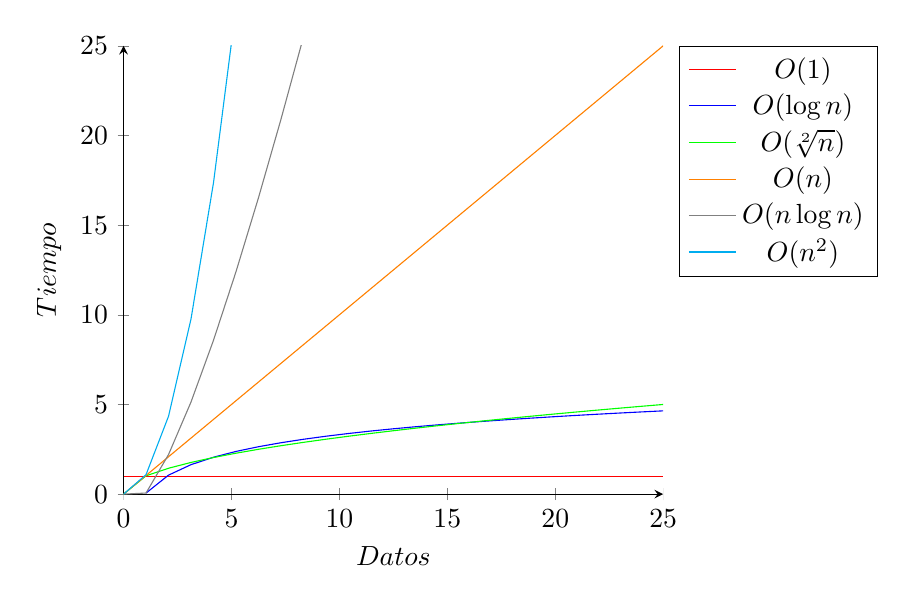
\begin{tikzpicture}[domain=0:25,samples=25]
    \begin{axis}[legend pos=outer north east,axis lines=left,xmin=0,xmax=25,ymin=0,ymax=25,xlabel={$Datos$},ylabel={$Tiempo$}]
    \addplot[color=red]{1};
    \addlegendentry{$O(1)$}
    \addplot[color=blue]{log2(x)};
    \addlegendentry{$O(\log n)$}
    \addplot[color=green]{sqrt(x)};
    \addlegendentry{$O(\sqrt[2]{n})$}
    \addplot[color=orange]{x};
    \addlegendentry{$O(n)$}
    \addplot[color=gray]{x*log2(x)};
    \addlegendentry{$O(n \log n)$}
    \addplot[color=cyan]{x^2};
    \addlegendentry{$O(n^2)$}
    \end{axis}
    \end{tikzpicture}
  \end{center}
\end{frame}

\subsection{Análisis de Algoritmos}

\begin{frame}{Análisis de algoritmos}
  \begin{itemize}
    \item Asumir que la cantidad de datos a procesar es un número grande.
    \item ¿Qué contar?
    \begin{itemize}
      \item Operaciones de comparación
      \item Operaciones aritméticas
      \item Copiado de datos
      \item Asignaciones
    \end{itemize}
    \item Tener conocimiento matemático
  \end{itemize}
\end{frame}

\begin{frame}[fragile]{...Análisis de algoritmos}
  \begin{itemize}
    \item Ejemplo: hallar el promedio de todos los números en el arreglo A.
	\begin{lstlisting}
int sum = 0;
int n = length(A);
for (int i=0; i < n; i++)
  sum = sum + A[i];
double prom = sum / n;
    \end{lstlisting}
    \begin{itemize}
      \item Tiempo detallado: $3 + 3n + 2 = 2n + 5$
      \item Tiempo asintótico: $O(n)$
    \end{itemize}
  \end{itemize}
\end{frame}

\begin{frame}[fragile]{Reglas para calcular el tiempo}
  \begin{itemize}
    \item Regla 1: sentencias secuenciales
    \item Cada operación y asignación tiene peso 1, funciones tienen su propio peso. Luego sumar todo.
    \begin{lstlisting}
i = x ----> 1
a = b + 2 * 3; ----> 3, 2 operaciones y una asignación
v[i] = v[0]; ----> 3, acceso a arreglos: 1 cada vez.
b = binarySearch(v, 10); ----> 1 + log n, búsqueda binaria: log(n)
cout << b; ----> 1, cout se puede asumir como tiempo 1
    \end{lstlisting}
    \begin{itemize}
      \item Tiempo detallado: $9 + \log n$
      \item Tiempo asintótico: $\log n$ $\longrightarrow$ Logarítmico
    \end{itemize}
  \end{itemize}
\end{frame}

\begin{frame}[fragile]{Reglas para calcular el tiempo}
  \begin{itemize}
    \item Regla 2: estructuras repetitivas
    \item Identificar el número de iteraciones y multiplicar por la expresión interior
    \begin{lstlisting}
for (int i = 0; i < n; ++i) { ----> n
  sum = sum + A[i]; ----> 3
  cout << sum; ----> 1
}
    \end{lstlisting}
    \begin{itemize}
      \item Tiempo detallado: $4n$
      \item Tiempo asintótico: $O(n)$ $\longrightarrow$ Lineal
    \end{itemize}
  \end{itemize}
\end{frame}


\begin{frame}[fragile]{Reglas para calcular el tiempo}
  \begin{itemize}
    \item Regla 3: repetitivas anidadas
    \begin{lstlisting}
for (int i = 0; i < n; ++i) { ----> n
  for (int k = 0; k < n; k += 2) { ----> n / 2
    cout << i * k; ----> 2
  }
}
    \end{lstlisting}
    \begin{itemize}
      \item Tiempo detallado: $\frac{n^2}{2}$
      \item Tiempo asintótico: $O(n^2)$ $\longrightarrow$ Cuadrático
    \end{itemize}
  \end{itemize}
\end{frame}

\begin{frame}[fragile]{Reglas para calcular el tiempo}
  \begin{itemize}
    \item Regla 4: repetitivas consecutivas
    \begin{lstlisting}
for (int i=0; i < n; i++) ----> n
  cout << i; ----> 1
for (int i = 0; i < n; ++i) { ----> n
  for (int k = 1; k < n; k *= 2) { ----> log n, en base 2
    cout << i * k; ----> 2
  }
}
    \end{lstlisting}
    \begin{itemize}
      \item Tiempo detallado: $ n + 2n\log n$
      \item Tiempo asintótico: $O(n\log n)$
    \end{itemize}
  \end{itemize}
\end{frame}

\begin{frame}[fragile]{Reglas para calcular el tiempo}
  \begin{itemize}
    \item Regla 5:  if ... else
    \item Escoger el máximo de la expresión verdadera y de la falsa
    \begin{lstlisting}
if (a > b) ---> máximo de: (1 + log n) y (2)
  a = binarySearch(v, b); ----> 1 + log n
else
  a = v[b]; ----> 2
    \end{lstlisting}
    \begin{itemize}
      \item Tiempo detallado: $1 + \log n$
      \item Tiempo asintótico: $O(\log n)$
    \end{itemize}
  \end{itemize}
\end{frame}

\begin{frame}{Tipos de análisis}
  \begin{itemize}
    \item Mejor caso (best case): si es que el input causa que tome el menor tiempo.
    \item Peor caso (worst case): da una idea del máximo tiempo que un algoritmo puede tomar.
    \item Caso promedio (average case): hay que tomar muchos detalles y aplicar algo de estadística para encontrar el tiempo esperado sobre todos los casos posibles del input.
  \end{itemize}
\end{frame}

\begin{frame}{¿Por qué medir la eficiencia de un algoritmo? }
  \begin{itemize}
    \item Nos ayuda a entender la escalabilidad.
    \item Nos permite discernir entre lo que es posible y lo imposible.
    \item Es un lenguaje que nos permite predecir el comportamiento de un programa.
    \item La eficiencia es la "moneda" en la computación.
    \item Buscar la rapidez de un programa es divertido! :D
    \item \alert{Debemos convertir esto en un hábito.}
  \end{itemize}
\end{frame}

\section{Referencias}
\begin{frame}{Referencias}
  \begin{thebibliography}{9}
    \bibitem{cormen}
    Thomas H. Cormen, Charles E. Leirserson, Ronald L. Rivest, Clifford Stein.
    \textbf{Introduction to Algorithms}.
    Third edition, The MIT Press, Cambridge, Massachusetts, 2009.
    \bibitem{pppcppt}
    Bjarne Stroustrup.
    \textbf{Programming: Principles and practice using C++}.
    Addison-Wesley, Upper Saddle River, NJ, Boston, 2009. Capítulo 19 sección 3, p. 656.
    \bibitem{isocppt}
    Standard C++ Foundation
    \textbf{Templates, C++ FAQ}. https://isocpp.org/wiki/faq/templates
  \end{thebibliography}
\end{frame}

\end{document}